Given our motivation of quickly benchmarking recommendation algorithms, we now aim to \emph{characterize} the performance of various commonly-used sampling strategies. We loosely define the performance of a sampling scheme as 
%it's
its
ability in effectively retaining the performance-ranking of different recommendation algorithms on the full \vs sub-sampled data. In this section, we start by discussing the different recommendation feedback scenarios we consider, along with a representative sample of popular recommendation algorithms that we aim to efficiently benchmark. We then examine popular data sampling strategies, followed by proposing a novel, proxy-based sampling strategy (\sampler) that is especially suited for sampling representative subsets from long-tail CF data.

\subsection{Problem Settings \& Methods Compared} \label{feedback_types} \label{algorithms}
To give a representative sample of typical recommendation scenarios, we consider three different user feedback settings. In \emph{explicit feedback}, each user $u$ gives a numerical rating $r^u_i$ to each interacted item $i$; the model must predict these ratings for novel (test) user-item interactions. Models from this class are evaluated in terms of the Mean Squared Error (MSE) of the predicted ratings. Another scenario we consider is \emph{implicit feedback}, where the interactions for each user are only available for positive items (\eg clicks or purchases), whilst all non-interacted items are considered as negatives. We employ the AUC, Recall@$100$, and nDCG@$10$ metrics to evaluate model performance for implicit feedback algorithms. Finally, we also consider \emph{sequential feedback}, where each user $u$ interacts with an ordered sequence of items $\mathcal{S}^u = (\mathcal{S}^u_1, \mathcal{S}^u_2, \ldots, \mathcal{S}^u_{|\mathcal{S}^u|})$ such that $\mathcal{S}^u_i \in \mathcal{I}$ for all $i \in \{1, \ldots, |\mathcal{S}^u|\}$. Given $\mathcal{S} = \{ \mathcal{S}^u ~|~ \forall u \in \mathcal{U} \}$, the goal is to identify the \emph{next-item} for each sequence $\mathcal{S}^u$ that each user $u$ is most likely to interact with. We use the same metrics as in implicit feedback settings. Note that following recent warnings against sampled metrics for evaluating recommendation algorithms \cite{sampled_metrics, castells_sampling}, we compute both Recall and nDCG by ranking \emph{all} items in the dataset. Further specifics about the datasets used, pre-processing, train/test splits, \etc are discussed in-depth in \cref{main_exp}. 

Given the diversity of the scenarios discussed above, there are numerous relevant recommendation algorithms. We use the following seven recommendation algorithms, intended to represent the state-of-the-art and standard baselines:
\begin{itemize}
    \listheader{PopRec:} A na\"ive baseline that simply ranks items according to overall train-set popularity. Note that this method is unaffected by the user for which items are being recommended, and has the \emph{same global ranking} of all items.
    
    \listheader{Bias-only:} Another simple baseline that assumes no interactions between users and items. Formally, it learns: (1) a global bias $\alpha$; (2) scalar biases $\beta_u$ for each user $u \in \mathcal{U}$; and (3) scalar biases $\beta_i$ for each item $i \in \mathcal{I}$. Ultimately, the rating/relevance for user $u$ and item $i$ is modeled as $\hat{r}^u_i = \alpha + \beta_u + \beta_i$.

    \listheader{Matrix Factorization (MF) \cite{mf}:} Represents both users and items in a common, low-dimensional latent-space by factorizing the user-item interaction matrix. Formally, the rating/relevance for user $u$ and item $i$ is modeled as $\hat{r}^u_i = \alpha + \beta_u + \beta_i + \gamma_u \cdot \gamma_i$ where $\gamma_u, \gamma_i \in \mathbb{R}^d$ are learned latent representations. 
    
    \listheader{Neural Matrix Factorization (NeuMF) \cite{neural_mf}:} Leverages the representation power of deep neural-networks to capture non-linear correlations between user and item embeddings. Formally, the rating/relevance for user $u$ and item $i$ is modeled as $\hat{r}^u_i = \alpha + \beta_u + \beta_i + f(\gamma_u ~||~ \gamma_i ~||~ \gamma_u \cdot \gamma_i)$ where $\gamma_u, \gamma_i \in \mathbb{R}^d$, `||' represents the concatenation operation, and $f : \mathbb{R}^{3d} \mapsto \mathbb{R}$ represents an arbitrarily complex neural network. 
    
    \listheader{Variational Auto-Encoders for Collaborative Filtering (MVAE) \cite{mvae}:} Builds upon the Variational Auto-Encoder (VAE) \cite{vae} framework to learn a low-dimensional representation of a user's consumption history. More specifically, MVAE encodes each user's bag-of-words consumption history using a VAE and further decodes the latent representation to obtain the completed user preference over all items.
    
    \listheader{Sequential Variational Auto-Encoders for Collaborative Filtering (SVAE) \cite{svae}:} A sequential algorithm that combines the temporal modeling capabilities of a GRU \cite{gru} along with the representation power of VAEs. Unlike MVAE, SVAE uses a GRU to encode the user's consumption sequence followed by a multinomial VAE at each time-step to model the likelihood of the next item. 
    
    \listheader{Self-attentive Sequential Recommendation (SASRec) \cite{sasrec}:} Another sequential algorithm that relies on the sequence modeling capabilities of self-attentive neural networks \cite{self_attention} to predict the occurance of the 
    %next-item 
    next item
    in a user's consumption sequence. To be precise, given a user $u$ and 
    %it's
    their
    time-ordered consumption history  $\mathcal{S}^u = (\mathcal{S}^u_1, \mathcal{S}^u_2, \ldots, \mathcal{S}^u_{|\mathcal{S}^u|})$, SASRec first applies self-attention on $\mathcal{S}^u$ followed by a series of non-linear feed-forward layers to finally obtain the next item likelihood.
\end{itemize}
We also list 
%the pertinence of 
models and metrics for each of the three different CF-scenarios in \cref{model_scenario_table}. Since bias-only, MF, and NeuMF can be trained for all three CF-scenarios, we optimize them using the regularized least-squares regression loss for explicit feedback, and the pairwise-ranking (BPR \cite{bpr}) loss for implicit/sequential feedback. Note however that the aforementioned algorithms are only intended to be a representative sample of a 
%wide-pool 
wide pool
of recommendation algorithms, and in our pursuit to benchmark recommender systems faster, we are primarily concerned with the \emph{ranking} of different algorithms on the full dataset \vs a smaller sub-sample.

\begin{table*}[!ht]
    \begin{small} % normalsize, small, footnotesize
    \begin{center}
        % \begin{subtable}{0.5\linewidth}
        % \centering
        %     \begin{tabular}{c | c c c}
        %         \toprule
        %         \multirow{2}{*}{Algorithm} & \multicolumn{3}{c}{CF-scenario} \\
        %         & Explicit & Implicit & Sequential \\ \midrule
                
        %         Bias-only   & Yes & Yes & Yes \\
        %         MF          & Yes & Yes & Yes \\
        %         NeuMF       & Yes & Yes & Yes \\
        %         PopRec      & $\times$ & Yes & Yes \\
        %         MVAE        & $\times$ & Yes & Yes \\
        %         SVAE        & $\times$ & $\times$ & Yes \\
        %         SASRec      & $\times$ & $\times$ & Yes \\ \bottomrule
        %     \end{tabular}
        % \end{subtable}%
        % \begin{subtable}{0.5\linewidth}
        % \centering
        %     \begin{tabular}{c | c c c}
        %         \toprule
        %         \multirow{2}{*}{Metric} & \multicolumn{3}{c}{CF-scenario} \\
        %         & Explicit & Implicit & Sequential \\ \midrule
                
        %         MSE       & Yes & $\times$ & $\times$ \\
        %         AUC       & $\times$ & Yes & Yes \\
        %         Recall@k  & $\times$ & Yes & Yes \\
        %         nDCG@k    & $\times$ & Yes & Yes \\ \bottomrule
        %     \end{tabular}
        % \end{subtable}%
        \begin{tabular}{c | c c c c c c c | c c c c}
            \toprule
            \multirow{3}{*}{CF-scenario} & \multicolumn{7}{c|}{\emph{Algorithm}} & \multicolumn{4}{c}{\emph{Metric}} \\
            & \multicolumn{7}{c|}{} & \multicolumn{4}{c}{} \\
            & Bias-only & MF & NeuMF & PopRec & MVAE & SVAE & SASRec & MSE & AUC & Recall@k & nDCG@k \\ \midrule
            Explicit & Yes & Yes & Yes & $\times$ & $\times$ & $\times$ & $\times$ & Yes & $\times$ & $\times$ & $\times$ \\[0.6mm]
            Implicit & Yes & Yes & Yes & Yes & Yes & $\times$ & $\times$ & $\times$ & Yes & Yes & Yes \\[0.6mm]
            Sequential & Yes & Yes & Yes & Yes & Yes & Yes & Yes & $\times$ & Yes & Yes & Yes \\[0.6mm]
            \bottomrule
        \end{tabular}
    \end{center}
    \end{small}
    \bigskip
    \caption{Demonstrates the pertinence of each CF-scenario towards each algorithm (left) and each metric (right). Note that we can use ranking metrics for explicit feedback, however, we only use MSE as a design choice and due to it's direct relevance.}
    \label{model_scenario_table}
    \vspace{-6mm} %Put here to reduce too much white space after your table
\end{table*}

\subsection{Sampling Strategies} \label{common_sampling_schemes}
Given a user-item CF dataset \dataset, we aim to create a $p\%$ subset $\mathcal{D}^{s, p}$ according to some sampling strategy $s$. In this paper, to be comprehensive, we consider a sample of eight popular sampling strategies, which can be grouped into the following three categories:

\subsubsection{Interaction sampling. \ \ } We first discuss three strategies that sample interactions from \dataset. In \emph{Random Interaction Sampling}, we generate $\mathcal{D}^{s, p}$ by randomly sampling $p\%$ of all the user-item interactions in \dataset. \emph{User-history Stratified Sampling} is another popular sampling technique (see \eg \cite{svae, handbook}) to generate smaller CF-datasets. To match the user-frequency distribution amongst \dataset and $\mathcal{D}^{s, p}$, it randomly samples $p\%$ of interactions from each user's consumption history. Unlike random stratified sampling, \emph{User-history Temporal Sampling} samples $p\%$ of the \emph{most recent} interactions for each user. This strategy is representative of the popular practice of making data subsets from the online traffic of the last $x$ days \cite{eclare, pfastre}.

\subsubsection{User sampling. \ \ } Similar to sampling interactions, we also consider two strategies which sample users in \dataset instead. To ensure a fair comparison amongst the different kinds of sampling schemes used in this paper, we retain exactly $p\%$ of the \emph{total interactions} in $\mathcal{D}^{s, p}$. In \emph{Random User Sampling}, we retain users from \dataset at random. To be more specific, we iteratively preserve \emph{all} the interactions for a random user until we have retained $p\%$ of the original interactions. Another strategy we employ is \emph{Head User Sampling}, in which we iteratively remove the user with the least amount of total interactions. This method is representative of commonly used data pre-processing strategies (see \eg \cite{mvae, neural_mf}) to make data suitable for parameter-heavy algorithms. Sampling the data in such a way can introduce bias toward users from minority groups which might raise concerns from a diversity and fairness perspective \cite{fairness}.

\subsubsection{Graph sampling. \ \ } Instead of sampling directly from \dataset, we also consider three strategies that sample from the inherent user-item bipartite interaction graph $\mathcal{G}$. In \emph{Centrality-based Sampling}, we proceed by computing the pagerank centrality scores \cite{pagerank} for each node in $\mathcal{G}$, and retain all the edges (interactions) of the \emph{top scoring nodes} until a total $p\%$ of the original interactions have been preserved. Another popular strategy we employ is \emph{Random-walk Sampling} \cite{large_graphs}, which performs multiple random-walks with restart on $\mathcal{G}$ and retains the edges amongst those pairs of nodes that have been visited at least once. We keep expanding our walk until $p\%$ of the initial edges have been retained. We also utilize \emph{Forest-fire Sampling} \cite{forest_fire}, which is a snowball sampling method and proceeds by randomly ``burning'' the outgoing edges of visited nodes. It initially starts with a random node, and then propagates to a random subset of previously unvisited neighbors. The propagation is terminated once we have created a graph-subset with $p\%$ of the initial edges.

\subsection{\sampler: Selection-Via-Proxy for CF data} \label{svp_cf} 
Selection-Via-Proxy (SVP) \cite{svp} is a leading coreset mining technique for classification datasets like CIFAR10 \cite{cifar} and ImageNet \cite{image_net}. The main idea proposed is simple and effective, and proceeds by training a relatively inexpensive base-model as a proxy to define the ``importance'' of a data-point. However, applying SVP to CF-data can be highly non-trivial because of the following impediments:
\begin{itemize}
    \listheader{Data heterogeneity:} Unlike classification data 
    % $\mathcal{D}_c = \left\{ (x, y) ~|~ x \in \mathbb{R}^d, y\in \mathcal{Y}\right\}$ 
    over some input space $\mathcal{X}$ and label-space $\mathcal{Y}$, CF-data consists of numerous four-tuples $\{u, i, r^u_i, t^u_i\}$. Such multimodal data adds many different dimensions to sample data from, making it increasingly complex to define meaningful samplers. 
    
    \listheader{Defining the importance of a data point:} Unlike classification, where we can measure the performance of a classifier by 
    %it's
    its
    empirical risk on held-out data, for recommendation, there are a variety of different scenarios (\cref{feedback_types}) along with a wide list of relevant evaluation metrics. Hence, it becomes challenging to adapt importance-tagging techniques like greedy k-centers \cite{k_centers}, forgetting-events \cite{forgetting_events}, \etc for recommendation tasks.
    
    \listheader{Missing data:} 
    CF-data is well-known for (1) 
    %it's 
    its
    sparsity; (2) skewed and long-tail user/item distributions; and (3) missing-not-at-random (MNAR) properties of the user-item interaction matrix. This results in additional problems as we are now sampling data from skewed, MNAR data, especially using proxy-models trained on the same skewed data. Such sampling in the worst-case might even lead to exacerbating existing biases in the data or even aberrant data samples.
\end{itemize}
To address these fundamental limitations in applying the SVP philosophy to CF-data, we propose \sampler to sample representative subsets from large user-item interaction data. \sampler is also specifically devised for our objective of benchmarking different recommendation algorithms, as it relies on the crucial assumption that the ``easiest'' part of a dataset will generally be easy \emph{for all} algorithms. Under this assumption, even after removing such data we are still likely to retain the overall algorithms' ranking.

Because of the inherent data heterogeneity in user-item interaction data, we can sub-sample in a variety of different ways. We design \sampler to be versatile in this aspect as it can be applied to sample users, items, interactions, or combinations of them, by marginally adjusting the definition of importance of each data-point. In this paper, we limit the discussion to only sampling users and interactions (separately), but extending \sampler for sampling across other data modalities should be relatively straightforward.

Irrespective of whether to sample users or interactions, \sampler proceeds by training an inexpensive proxy model $\mathcal{P}$ on the full, original data \dataset and modifies the forgetting-events approach \cite{forgetting_events} to retain the points with the \emph{highest} importance. To be more specific, for explicit feedback, we define the importance of each data-point \ie $\{u, i, r^u_i, t^u_i\}$ interaction as $\mathcal{P}$'s average MSE (over epochs) of the specific interaction if we're sampling interactions \emph{or} $\mathcal{P}$'s average MSE of $u$ (over epochs) if we're sampling users. Whereas, for implicit and sequential feedback, we use $\mathcal{P}$'s average inverse-AUC while computing the importance of each data-point. For the sake of completeness, we experiment with both Bias-only and MF as two different kinds of proxy-models for \sampler. Since both models can be trained for all three CF-scenarios (\cref{model_scenario_table}), we can directly use them to tag the importance for each CF-scenario.

Ultimately, to handle the MNAR and long-tail problems, we also propose \samplerprop which employs user and item propensities to correct the distribution mismatch while estimating the importance of each datapoint. More specifically, let $p_{u, i} = P(r^u_i = 1 ~|~ \overstar{r}^u_i = 1)$ denote the probability of user $u$ and item $i$'s interaction actually being observed (propensity), $E$ be the total number of epochs that $\mathcal{P}$ was trained for, $\mathcal{P}_e$ denote the proxy model after the $e^{\mathit{th}}$ epoch, $\mathcal{I}_u^+ \coloneqq \{ j ~|~ r^u_j > 0 \}$ be the set of positive interactions for $u$, and $\mathcal{I}_u^- \coloneqq \{ j ~|~ r^u_j = 0 \}$ be the set of negative interactions for $u$; then, the importance function for \samplerprop, $\mathcal{I}_p$ is defined as follows:
\begin{align*}
% \begin{gathered}
    \mathcal{I}_p(u ~|~ \mathcal{P}) \coloneqq \frac{1}{|\mathcal{I}_u^+|} \cdot \sum_{i \in \mathcal{I}_u^+} \mathcal{I}_p(u, i ~|~ \mathcal{P}) \hspace{0.63em} ; \hspace{0.63em}
    \mathcal{I}_p(u, i ~|~ \mathcal{P}) \coloneqq \frac{\Delta(u, i ~|~ \mathcal{P})}{p_{u, i}} \\
    %where, 
% \end{gathered}
\end{align*}
\vspace{-0.6cm}
\begin{equation*}
\begin{gathered}
    \text{where,}
    \qquad \Delta(u, i ~|~ \mathcal{P}) \coloneqq 
    \begin{dcases} 
      ~~ \sum_{e=1}^{E} \left(\mathcal{P}_e(u, i) - r^u_i\right)^2 \\  %& \, \text{for explicit feedback} \\
      ~~ \text{(for explicit feedback)} \\ \\
      ~~ \sum_{e=1}^{E} \sum_{j \sim \mathcal{I}_u^-} \frac{1}{\mathds{1}\left(\mathcal{P}_e(u, i) > \mathcal{P}_e(u, j)\right)} \\ % & \, \text{for implicit/sequential feedback}
      ~~ \text{(for implicit/sequential feedback)}
   \end{dcases}
\end{gathered}
\end{equation*}
\vspace{0.1cm}

\begin{proposition}
Given an ideal propensity-model $p_{u, i}; \ \mathcal{I}_p(u, i ~|~ \mathcal{P})$ is an unbiased estimator of $\Delta(u, i ~|~ \mathcal{P})$.
\end{proposition}

\begin{proof}
\begin{align*}
    \EE_{u \sim \mathcal{U}} \EE_{i \sim \mathcal{I}} \left[ \mathcal{I}_p(u, i ~|~ \mathcal{P}) \right] \hspace{5.65cm}
\end{align*}
\vspace{-0.4cm}
\begin{align*}
    &= \frac{1}{|\mathcal{U}| |\mathcal{I}|} \sum_{u \sim \mathcal{U}} \sum_{i \sim \mathcal{I}} \mathcal{I}_p(u, i ~|~ \mathcal{P}) \cdot P(r_i^u = 1) \\
    % &= \frac{1}{|\mathcal{U}| \cdot |\mathcal{I}|} \sum_{u \sim \mathcal{U}} \sum_{i \sim \mathcal{I}} \mathcal{I}_p(u, i ~|~ \mathcal{P}) \cdot \left( P(r_i^u = 1, \overstar{r}_i^u = 0) ~+~ P(r_i^u = 1, \overstar{r}_i^u = 1) \right) \\
    &= \begin{aligned}[t]
        \frac{1}{|\mathcal{U}| |\mathcal{I}|} \sum_{u \sim \mathcal{U}} \sum_{i \sim \mathcal{I}} \frac{\Delta(u, i ~|~ \mathcal{P})}{p_{u, i}} \cdot ( P(\overstar{r}_i^u = 0) \cdot \cancelto{0}{P(r_i^u = 1 ~|~ \overstar{r}_i^u = 0)} \\
        +~ P(\overstar{r}_i^u = 1) \cdot P(r_i^u = 1 ~|~ \overstar{r}_i^u = 1)) \\ % \hspace{3.6cm} \\
        % \text{(One-sided label noise)} \\
    \end{aligned} \\
    &= \frac{1}{|\mathcal{U}| |\mathcal{I}|} \sum_{u \sim \mathcal{U}} \sum_{i \sim \mathcal{I}} \Delta(u, i ~|~ \mathcal{P}) \cdot P(\overstar{r}_i^u = 1) \\ %\hspace{0.5cm} 
    &= \EE_{u \sim \mathcal{U}} \EE_{i \sim \mathcal{I}} \left[ \Delta(u, i ~|~ \mathcal{P}) \right] \qedhere
\end{align*}
\end{proof} 

\paragraph{Propensity model.} A wide variety of ways exist 
%in the literature 
to model the propensity score of a user-item interaction \cite{propensity_1, rec_as_treatments, sachdeva_kdd20, pfastre}. The most common ways comprise using machine learning models like na\"ive bayes and logistic regression \cite{rec_as_treatments}, or by fitting handcrafted functions \cite{pfastre}. For our problem statement, we make a simplifying assumption that the data noise is one-sided \ie $P(r^u_i = 1 ~|~ \overstar{r}^u_i = 0)$ or the probability of a user interacting with a \emph{wrong} item is \emph{zero}, and model the probability of an interaction going missing to decompose over the user and item as follows:
\begin{align*}
    p_{u, i} &= P(r^u_i = 1 ~|~ \overstar{r}^u_i = 1) \\
    &= P(r^u = 1 ~|~ \overstar{r}^u = 1) \cdot P(r_i = 1 ~|~ \overstar{r}_i = 1) ~=~ p_u \cdot p_i
\end{align*}
% \begin{equation}
%     p_{u, i} \ \ = \ \ P(r^u_i = 1 ~|~ \overstar{r}^u_i = 1)
%     \ \ = \ \ P(r^u = 1 ~|~ \overstar{r}^u = 1) \cdot P(r_i = 1 ~|~ \overstar{r}_i = 1) 
%     \ \ = \ \ p_u \cdot p_i
% \end{equation}
Ultimately, following \cite{pfastre}, we assume the user and item propensities to lie on the following sigmoid curves:
\begin{equation*}
\begin{split}
    p_u \coloneqq \frac{1}{1 + C_u \cdot e^{-A \cdot log(N_u + B)}} \quad ; \quad p_i \coloneqq \frac{1}{1 + C_i \cdot e^{-A \cdot log(N_i + B)}}
\end{split}
\end{equation*}
Where, $N_u$ and $N_i$ represent the total number of interactions of user $u$ and item $i$ respectively, $A$ and $B$ are two fixed scalars, $C_u = (log(|\mathcal{U}|) - 1) \cdot (B+1)^A$ and $C_i = (log(|\mathcal{I}|) - 1) \cdot (B+1)^A$. 

\subsection{Performance of a sampling strategy} \label{sampling_perf}
% Preserving \emph{exactly} the same levels of performance on sub-sampled data over metrics like MSE, AUC, \etc is a very challenging problem. However, a simpler albeit useful problem is accurately preserving the \emph{ranking} of different algorithms on sub-sampled data. For \eg, a sampling scheme that has a very low bias but high variance in preserving metric performance values has a lesser utility than a different sampling scheme with high amounts of bias but low variance, since the algorithm ranking is still preserved and can be used to benchmark models much faster. With the following notion in mind, to 
To quantify the performance of a sampling strategy $s$ on a dataset $\mathcal{D}$, we start by creating various $p\%$ subsets of $\mathcal{D}$ according to $s$ and call them $\mathcal{D}^{s, p}$. Next, we train and evaluate all the relevant recommendation algorithms on both $\mathcal{D}$ and $\mathcal{D}^{s, p}$. Let the \emph{ranking} of all algorithms according to CF-scenario $f$ and metric $m$ trained on $\mathcal{D}$ and $\mathcal{D}^{s, p}$ be $\mathcal{R}_{f, m}$ and $\mathcal{R}^{s, p}_{f, m}$ respectively, then the performance measure $\Psi(\mathcal{D}, s)$ is defined as the average correlation between $\mathcal{R}_{f, m}$ and $\mathcal{R}^{s, p}_{f, m}$ measured through Kendall's Tau over all possible CF-scenarios, metrics, and sampling percents:
\begin{equation*}
\begin{split}
    \Psi\left(\mathcal{D}, s\right) &= \lambda \cdot \sum_{f} \sum_{m} \sum_{p} \tau\left(\mathcal{R}_{f, m}, \mathcal{R}^{s, p}_{f, m}\right) \\
    % &= \lambda \cdot \sum_{f} \sum_{m} \sum_{p} \frac{2}{n \cdot (n-1)} \sum_{i < j} \mathds{1}\left(\mathcal{R}_{f, m}(i) - \mathcal{R}_{f, m}(j)\right) \cdot \mathds{1}\left(\mathcal{R}^{s, p}_{f, m}(i) - \mathcal{R}^{s, p}_{f, m}(j)\right)
\end{split}
\end{equation*}
Where $\lambda$ is an appropriate normalizing constant for computing the average, sampling percent $p \in \{ 80, 60, 40, 20, 10, 1 \}$, CF-scenario $f$, metric $m$ and their pertinence towards each other can all be found in \cref{model_scenario_table}. $\Psi$ has the same range as Kendall's Tau \ie $[-1, 1]$ and a higher $\Psi$ indicates strong agreement between the algorithm ranking on the full and sub-sampled datasets, whereas a large negative $\Psi$ implies that the algorithm order was effectively reversed.

\subsection{Experiments} \label{main_exp}

\paragraph{Datasets.} To promote dataset diversity in our experiments, we use six public user-item rating interaction datasets with varying sizes, sparsity patterns, and other characteristics. We use the Magazine, Luxury, and Video-games categories of the Amazon review dataset \cite{amz_data}, along with the Movielens-100k \cite{movielens}, BeerAdvocate \cite{beer_dataset}, and GoodReads Comics \cite{mengting_goodreads} datasets. A brief set of data statistics is also presented in \cref{data_stats}. We simulate all three CF-scenarios (\cref{feedback_types}) 
% for each dataset 
via different pre-processing strategies. For explicit and implicit feedback, we follow a randomized 80/10/10 train-test-validation split for each user's consumption history in the dataset, and make use of the leave-one-last \cite{train_test_splitting} strategy for sequential feedback \ie
% leave the last interaction in each user's time-sorted consumption history as a testing-point and the second last interaction as a validation-point. 
keep the last two interactions in each user's time-sorted consumption history in the validation and test-set respectively.
Since we can't control the initial construction of datasets, and to minimize the initial data bias, we follow the least restrictive data pre-processing \cite{making_progress, sigir20}. We only weed out the users 
% that have lesser 
with less
than 3 interactions,
% in total, in order 
to keep at least one occurrence 
% per user 
in the train, validation, and test sets.

\begin{table}[!ht]
    % \vspace{-1mm} %Put here to reduce too much white space after your table
    \begin{footnotesize} % normalsize, small, footnotesize
    \begin{center}
        \begin{tabular}{c | c c c c}
            \toprule
            \multirow{2}{*}{\textbf{Dataset}} & \textbf{\#} & \textbf{\#} & \textbf{\#} & \textbf{Avg. User} \\ 
            & \textbf{Interactions} & \textbf{Users} & \textbf{Items} & \textbf{history length} \\
            \midrule
            
            Amazon Magazine      & 12.7k & 3.1k  & 1.3k  & 4.1 \\
            ML-100k              & 100k  & 943   & 1.7k  & 106.04 \\
            Amazon Luxury        & 126k  & 29.7k & 8.4k  & 4.26 \\
            Amazon Video-games   & 973k  & 181k  & 55.3k & 5.37 \\
            BeerAdvocate         & 1.51M & 18.6k & 64.3k & 81.45 \\
            Goodreads Comics     & 4.37M & 133k  & 89k   & 32.72 \\
            
            \bottomrule
        \end{tabular}
    \end{center}
    \end{footnotesize}
    \vspace{2mm}
    \caption{Data statistics of the \emph{six} datasets used in this paper.}
    \label{data_stats}
    \vspace{-6mm} %Put here to reduce too much white space after your table
\end{table}

\paragraph{Training details.} We implement all algorithms in PyTorch\footnote{Code is available at \href{https://github.com/noveens/sampling_cf}{\color{blue}{https://github.com/noveens/sampling\_cf}}} 
and train on a single GPU. For a fair comparison across algorithms, we perform 
%a generous 
hyper-parameter search on the validation set. 
For the three smallest datasets used in this paper (\cref{data_stats}), we search the latent size in $\{ 4, 8, 16, 32, 50 \}$, dropout in $\{ 0.0, 0.3, 0.5 \}$, and the learning rate in $\{ 0.001, 0.006, 0.02 \}$. Whereas for the three largest datasets, we fix the learning rate to be $0.006$. % and only search over the latent-size and dropout values. 
Note that despite the limited number of datasets and recommendation algorithms used in this study, given that we need to train all algorithms with hyper-parameter tuning for all CF scenarios, $\%$ data sampled according to all different sampling strategies discussed in \cref{common_sampling_schemes}, there are a total of 
% $6 \times 3 \times 7 \times 16 \times 7 \times 30 \approx 400k$ 
$\sim400k$ 
unique models trained, 
% resulting in 
equating to
a cumulative train time of over $400k ~ \times \sim1 \text{min} \approx 9$ months.

\paragraph{Data sampling.} To compute the $\Psi$-values as defined in \cref{sampling_perf}, we construct $\{ 80, 60, 40, 20, 10, 1 \} \%$ samples for each dataset and sampling strategy. To keep comparisons as fair as possible, for all sampling schemes, we only sample on the train set and never touch the validation and test sets. % This simulates the practical scenario of sampling data only while benchmarking algorithms offline, whereas the live (test-set) traffic still remains the same.

\subsubsection{How do different sampling strategies compare to each other? \ \ } Results with $\Psi$-values for all sampling schemes on all datasets are in \cref{psi_results}. Even though there are only six datasets under consideration, there are a few prominent patterns. First, the average $\Psi$ for most sampling schemes is around $0.4$, which implies a statistically significant correlation between the ranking of algorithms on the full \vs sub-sampled datasets. Next, \sampler generally outperforms all commonly used sampling strategies by some margin in retaining the ranking of different recommendation algorithms. Finally, the methods that discard the tail of a dataset (head-user and centrality-based) are the worst performing strategies overall, which supports the recent warnings against dense sampling of data \cite{sigir20}.

\newcommand{\STAB}[1]{\begin{tabular}{@{}c@{}}#1\end{tabular}}
\begin{table*}%[!ht]
    \begin{footnotesize}
    \begin{center}
        \begin{tabular}{c c | c c c c c c | c}
            \toprule
            \multicolumn{2}{c|}{\multirow{4}{*}{\textbf{Sampling strategy}}} & \multicolumn{6}{c|}{\emph{Datasets}} & \\
            & & \multicolumn{6}{c|}{} & \\
            & & \begin{tabular}{@{}c@{}}\textbf{Amazon}\\\textbf{Magazine}\end{tabular} & \textbf{ML-100k} & \begin{tabular}{@{}c@{}}\textbf{Amazon}\\\textbf{Luxury}\end{tabular} & \begin{tabular}{@{}c@{}}\textbf{Amazon}\\\textbf{Video-games}\end{tabular} & \textbf{BeerAdvocate} & \begin{tabular}{@{}c@{}}\textbf{Goodreads}\\\textbf{Comics}\end{tabular} & \textbf{\emph{Average}} \\
            \midrule
            
            \multirow{8}{*}{\STAB{\rotatebox[origin=c]{90}{\begin{tabular}{@{}c@{}}Interaction sampling\\\end{tabular}}}} & Random & 0.428     &  0.551     &  0.409     &  0.047     &  0.455     &  0.552     &  0.407 \\[0.6mm]
            & Stratified & 0.27      &  0.499     &  0.291     &  -0.01     &  0.468     &  0.538     &  0.343 \\[0.6mm]
            & Temporal & 0.289     &  0.569     &  0.416     &  -0.02     &  \underline{0.539}     &  0.634     &  0.405 \\[0.6mm]
            & \sampler \emph{w/} MF & 0.418     &  0.674     &  0.398     &  0.326     &  0.425     &  \underline{0.662}     &  \underline{0.484} \\[0.6mm]
            & \sampler \emph{w/} Bias-only & 0.38      &  0.684     &  \underline{0.431}     &  \underline{0.348}     &  0.365     &  0.6       &  0.468 \\[0.6mm]
            & \samplerprop \emph{w/} MF & 0.381     &  0.617     &  0.313     &  0.305     &  0.356     &  0.608     &  0.43 \\[0.6mm]
            & \samplerprop \emph{w/} Bias-only & 0.408     &  0.617     &  0.351     &  0.316     &  0.437     &  0.617     &  0.458 \\[0.6mm]
            \midrule
            \multirow{7}{*}{\STAB{\rotatebox[origin=c]{90}{\begin{tabular}{@{}c@{}}User sampling\\\end{tabular}}}} & Random & 0.436     &  0.622     &  0.429     &  0.17      &  0.344     &  0.582     &  0.431 \\[0.6mm]
            & Head & 0.369     &  0.403     &  0.315     &  0.11      &  -0.04     &  -0.02     &  0.19 \\[0.6mm]
            & \sampler \emph{w/} MF & 0.468     &  0.578     &  0.308     &  0.13      &  0.136     &  0.444     &  0.344 \\[0.6mm]
            & \sampler \emph{w/} Bias-only & 0.49      &  0.608     &  0.276     &  0.124     &  0.196     &  0.362     &  0.343 \\[0.6mm]
            & \samplerprop \emph{w/} MF & 0.438 &  0.683 &  0.307 &  0.098 &  0.458 &  0.592 &  0.429 \\[0.6mm]
            & \samplerprop \emph{w/} Bias-only & 0.434     &  \underline{0.751}     &  0.233     &  0.107     &  0.506     &  0.637     &  0.445 \\[0.6mm]
            \midrule
            \multirow{4}{*}{\STAB{\rotatebox[origin=c]{90}{\begin{tabular}{@{}c@{}}Graph\\\end{tabular}}}} & Centrality & 0.307     &  0.464     &  0.407     &  0.063     &  0.011     &  0.343     &  0.266 \\[0.6mm]
            & Random-walk & \underline{0.596}  &  0.5       &  0.395     &  0.306     &  0.137     &  0.442     &  0.396 \\[0.6mm]
            & Forest-fire & 0.564  &  0.493   &  0.415   &  0.265   &  0.099  &  0.454  &  0.382 \\[0.6mm]
            \bottomrule
        \end{tabular}
        % \begin{tabular}{c || c c c | c c | c c c}
        %     \toprule
        %     \multirow{3}{*}{Dataset} & \multicolumn{3}{c|}{Interaction sampling} & \multicolumn{2}{c|}{User sampling} & \multicolumn{3}{c}{Graph sampling} \\
        %     \multirow{2}{*}{} & \multicolumn{3}{c|}{} & \multicolumn{2}{c|}{} & \multicolumn{3}{c}{} \\
        %     & Random & Stratified & Temporal & Random & Head & Centrality & RW & FF \\ \midrule \midrule
            
        %     Amazon Magazine     & 0.428    & 0.27     & 0.289    & 0.436    & 0.369    & 0.307    & \underline{0.596} & 0.564 \\
        %     ML-100k             & 0.551    & 0.499    & 0.569    & 0.622    & 0.403    & 0.464    & 0.5      & 0.493 \\
        %     Amazon Luxury       & 0.409    & 0.291    & 0.416    & 0.429    & 0.315    & 0.407    & 0.395    & 0.415 \\
        %     Amazon Video-games  & 0.047    & -0.01    & -0.02    & 0.17     & 0.11     & 0.063    & 0.306    & 0.265 \\
        %     BeerAdvocate        & 0.455    & 0.468    & \underline{0.539}    & 0.344    & -0.04    & 0.011    & 0.137    & 0.099 \\
        %     Goodreads Comics    & 0.552    & 0.538    & 0.634    & 0.582    & -0.02    & 0.343    & 0.442    & 0.454 \\ \midrule
        %     Average             & 0.407    & 0.343    & 0.405    & 0.431    & 0.19     & 0.266    & 0.396    & 0.382 \\ \bottomrule 
        % \end{tabular}
        % \newline
        % \vspace*{0.5 cm}
        % \newline
        % \begin{tabular}{c || c c c c | c c c c}
        %     \toprule
        %     \multirow{4}{*}{Dataset} & \multicolumn{4}{c|}{Interaction sampling} & \multicolumn{4}{c}{User sampling} \\
        %     \multirow{2}{*}{} & \multicolumn{4}{c|}{} & \multicolumn{4}{c}{} \\
        %     & SVP-CF & SVP-CF-Prop & SVP-CF & SVP-CF-Prop & SVP-CF & SVP-CF-Prop & SVP-CF & SVP-CF-Prop \\
        %     & Bias-only & Bias-only & MF & MF & Bias-only & Bias-only & MF & MF \\ \midrule \midrule
            
        %     Amazon Magazine     & 0.38     & 0.408    & 0.418    & 0.381    & 0.49     & 0.434    & 0.468    & 0.438 \\
        %     ML-100k             & 0.684    & 0.617    & 0.674    & 0.617    & 0.608    & \underline{0.751}    & 0.578    & 0.683 \\
        %     Amazon Luxury       & \underline{0.431}    & 0.351    & 0.398    & 0.313    & 0.276    & 0.233    & 0.308    & 0.307 \\
        %     Amazon Video-games  & \underline{0.348}    & 0.316    & 0.326    & 0.305    & 0.124    & 0.107    & 0.13     & 0.098 \\
        %     BeerAdvocate        & 0.365    & 0.437    & 0.425    & 0.356    & 0.196    & 0.506    & 0.136    & 0.458 \\
        %     Goodreads Comics    & 0.6      & 0.617    & \underline{0.662}    & 0.608    & 0.362    & 0.637    & 0.444    & 0.592 \\ \midrule 
        %     Average             & 0.468    & 0.458    & \underline{0.484}    & 0.43     & 0.343    & 0.445    & 0.344    & 0.429 \\ \bottomrule
        % \end{tabular}
    \end{center}
    \end{footnotesize}
    \bigskip
    \caption{$\Psi$-values for all datasets and sampling strategies. Higher $\Psi$ is better. The best $\Psi$ for every dataset is \underline{underlined}. The $\Psi$-values for each sampling scheme \emph{averaged over all datasets} is appended to the right.}
    \label{psi_results}
    \vspace{-6mm} %Put here to reduce too much white space after your table
\end{table*}

\subsubsection{How does the relative performance of algorithms change as a function of sampling rate? \ \ } In an attempt to better understand the impact of sampling on different recommendation algorithms used in this study (\cref{algorithms}), we visualize the probability of a recommendation algorithm moving up in the overall method ranking with data sampling. We estimate the aforementioned probability using Maximum-Likelihood-Estimation (MLE) on the experiments already run in computing $\Psi(\mathcal{D}, s)$. Formally, given a recommendation algorithm $r$, CF-scenario $f$, and data sampling percent $p$:
\begin{equation*}
    P_{\mathit{MLE}}(r ~|~ f, p) = \lambda \cdot \sum_{\mathcal{D}} \sum_{s} \sum_{m} 0.5 + \frac{\mathcal{R}_{f, m}(r) - \mathcal{R}_{f, m}^{s, p}(r)}{2 \cdot (n-1)}
\end{equation*}
where $\lambda$ is an appropriate normalizing constant, and $n$ represents the total number of algorithms. A heatmap visualizing $P_{\mathit{MLE}}$ for all algorithms and CF-scenarios is shown in \cref{percent_sampling_vs_method}. We see that simpler methods like Bias-only and PopRec have the highest probability across data scenarios of increasing their ranking order with extreme sampling. Whereas parameter-heavy algorithms like SASRec, SVAE, MVAE, \etc tend to decrease in the ranking order, which is indicative of overfitting on smaller data samples.
\begin{figure}[ht!]     
    \centering
    \vspace{-0.1cm}
    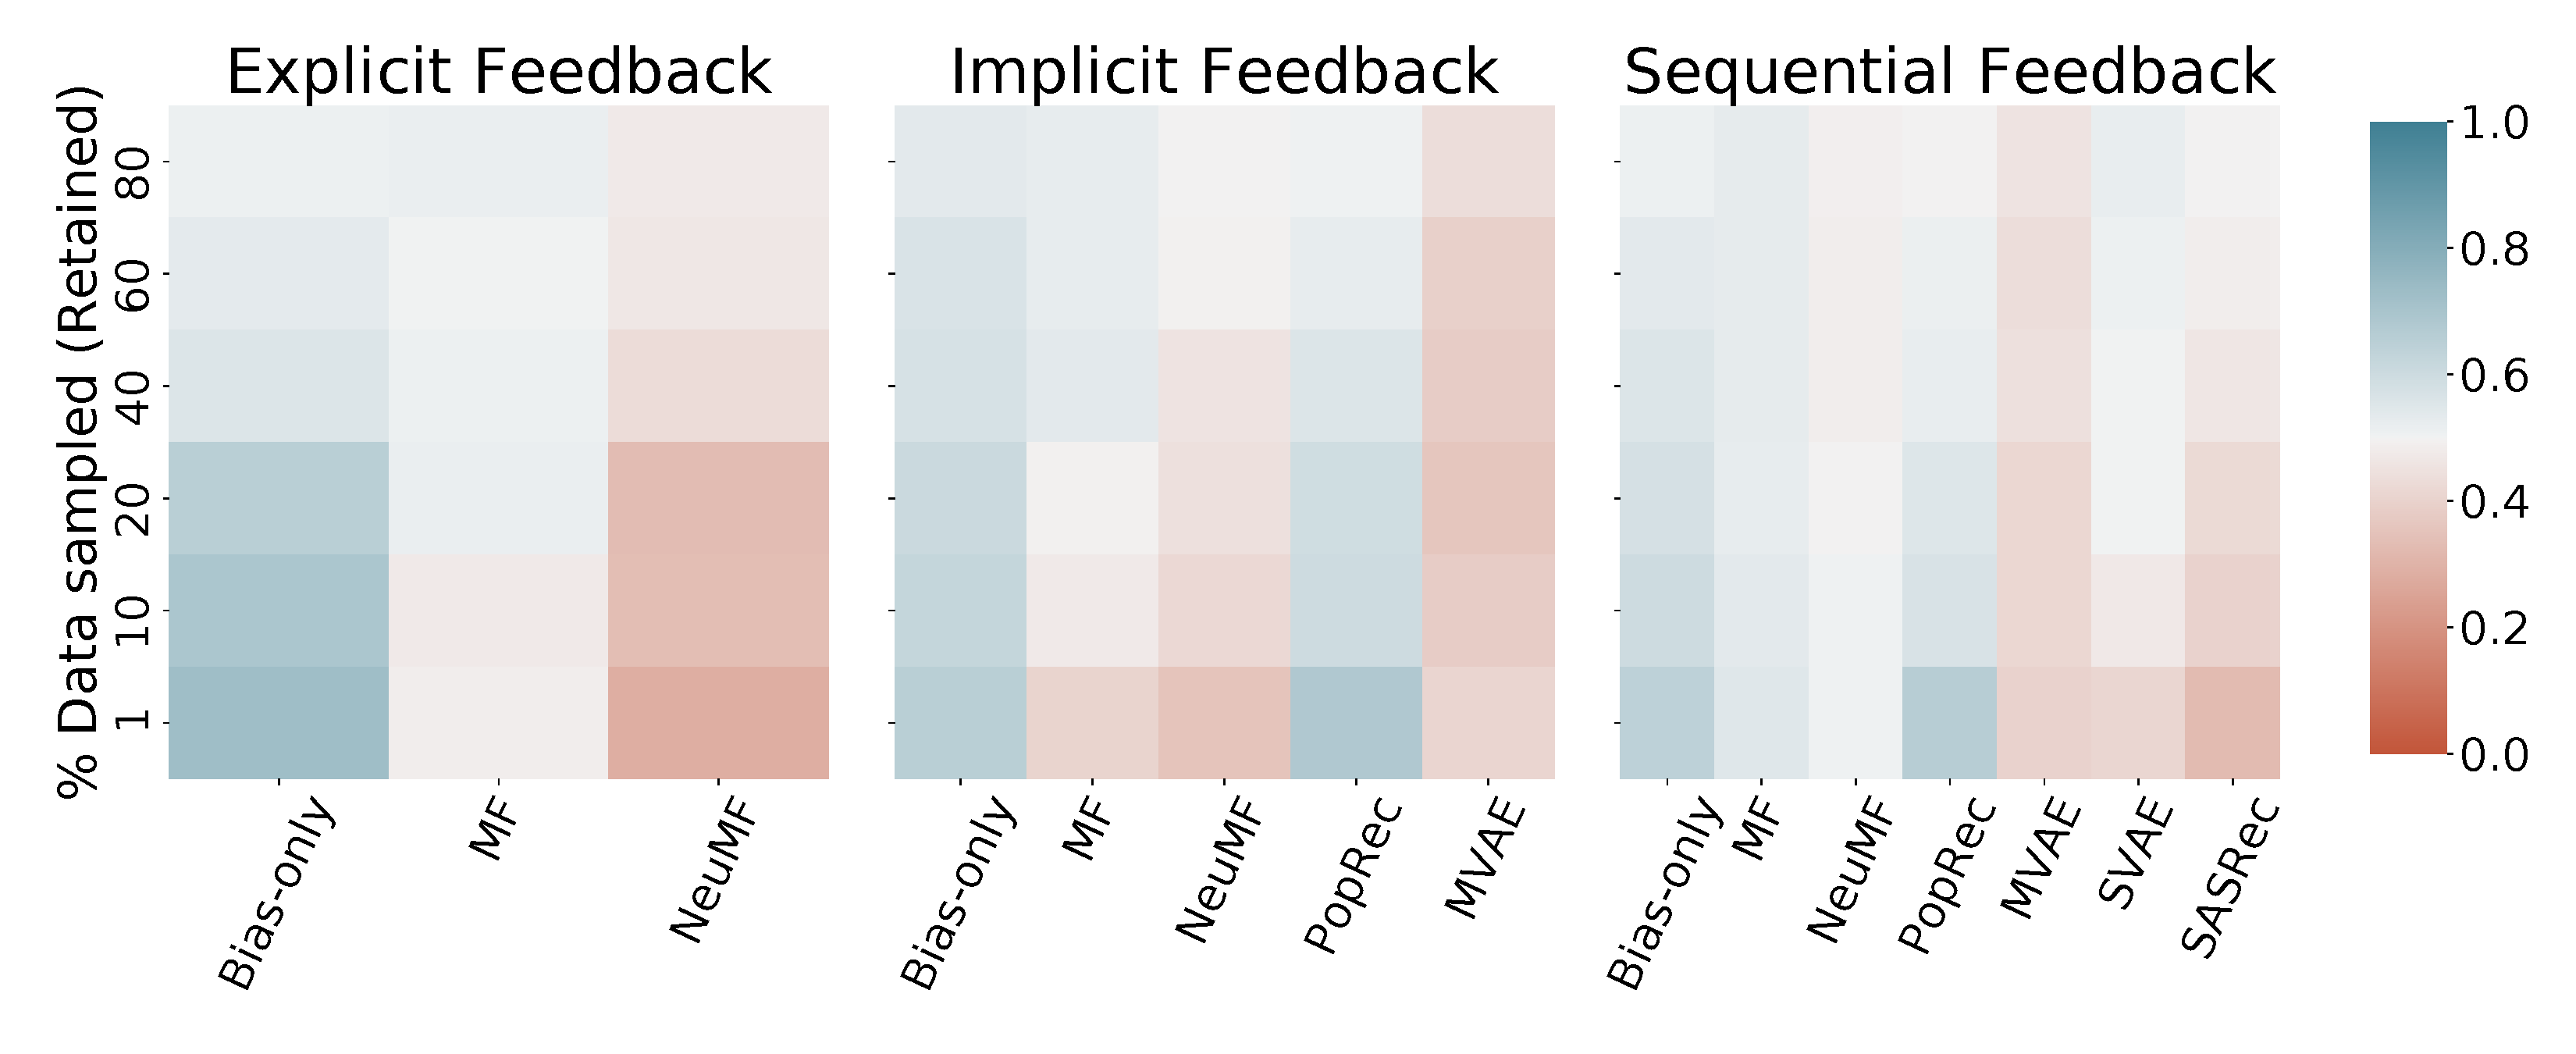
\includegraphics[width=0.9\linewidth]{figures/percent_sampling_vs_method.pdf}
    \vspace{-0.4cm}
    \caption{Heatmap of the probability of an algorithm moving in the overall ranking with extreme sampling. A high value indicates that the algorithm is most probable to \emph{move up} in the sampled data ranking order, whereas a low value indicates that the algorithm is most probable to \emph{move down}.}
    \label{percent_sampling_vs_method}
    \vspace{-0.3cm}
\end{figure}

\subsubsection{How much data to sample? \ \ } Since $\Psi$ is averaged over all $p \in \{ 80, 60, 40, 20, 10, 1 \}$\% data samples, to better estimate a reasonable amount of data to sample, we stratify $\Psi$ according to each value of $p$ and note the average Kendall's Tau. As we observe from \cref{percent_sampling_vs_tau}, %there is an expected, 
there is a steady increase in the performance measure when more data is retained. Next, despite the results in \cref{percent_sampling_vs_tau} being averaged over \emph{sixteen} sampling strategies, we still notice a significant amount of performance retained after sampling just $50-60\%$ of the data. % This holds to show that sampled data in some conditions can accurately reflect true algorithm performance.
\begin{figure}[ht!] 
    \centering
    \vspace{-0.2cm}
    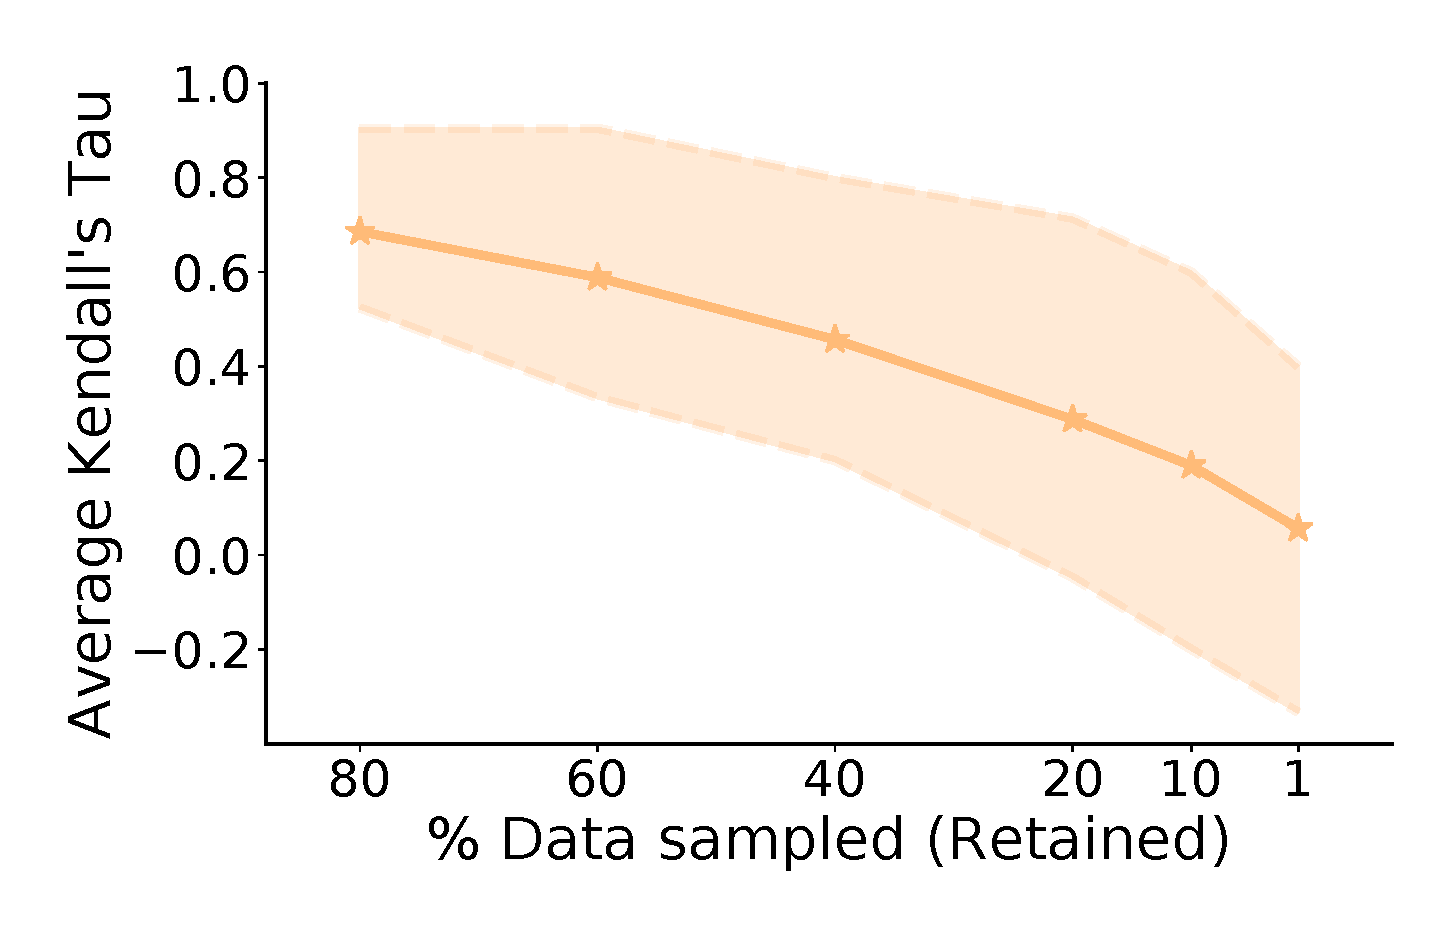
\includegraphics[width=0.6\linewidth]{figures/percent_sampling_vs_tau.pdf}
    \vspace{-0.25cm}
    \caption{Comparison of the average Kendall's Tau with \% data sampled. A higher Tau indicates better retaining power of the ranking of different recommendation algorithms.}
    \label{percent_sampling_vs_tau}
    \vspace{-0.3cm}
\end{figure} 

\subsubsection{Are different metrics affected equally by sampling? \ \ } In an attempt to better understand how the different implicit and sequential feedback metrics (\cref{feedback_types}) are affected by sampling, we visualize the average Kendall's Tau for all sampling strategies (except \sampler for brevity) and all \% data sampling choices separately over the AUC, Recall, and nDCG metrics in \cref{metric_correlation}. As expected, we observe a steady decrease in the model quality across the accuracy metrics over the different sampling schemes. This is in agreement with the analysis from \cref{percent_sampling_vs_tau}. Next, most sampling schemes follow a \emph{similar} downwards trend in performance for the three metrics with AUC being slightly less affected and nDCG being slightly more affected by extreme sampling.
\begin{figure}[ht!] 
    \vspace{-0.1cm}
    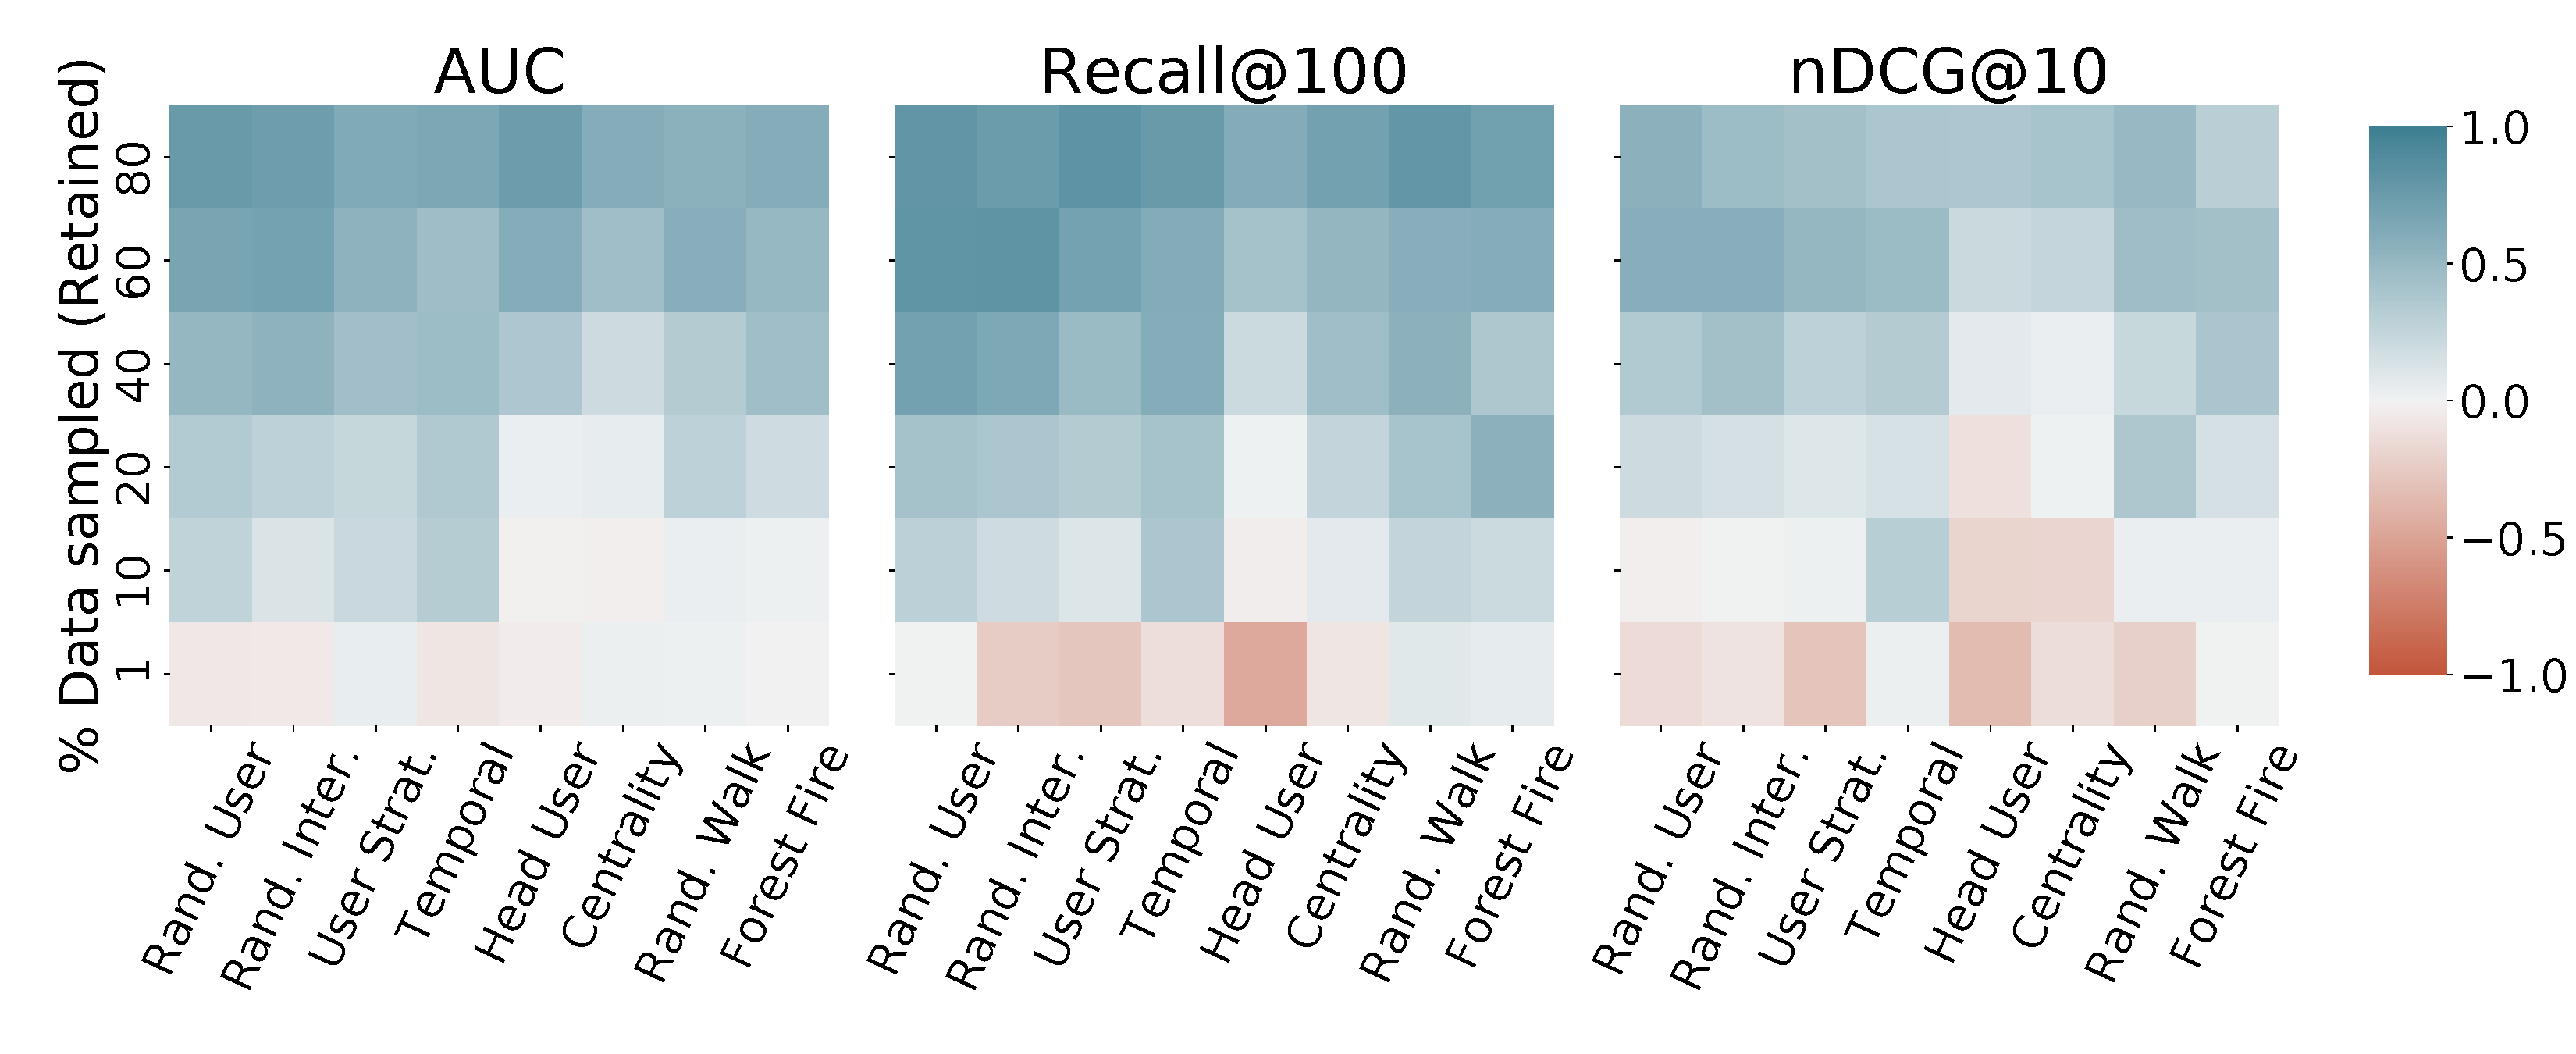
\includegraphics[width=\linewidth]{figures/percent_sampling_vs_sampler.pdf}
    \vspace{-0.8cm}
    \caption{Heatmap of the average Kendall's Tau for different samplers stratified over metrics and \% data sampled.}
    \label{metric_correlation}
    \vspace{-0.5cm}
\end{figure}
% \begin{wrapfigure}{r}{0.36\textwidth}
%     \vspace{-0.3cm}
%     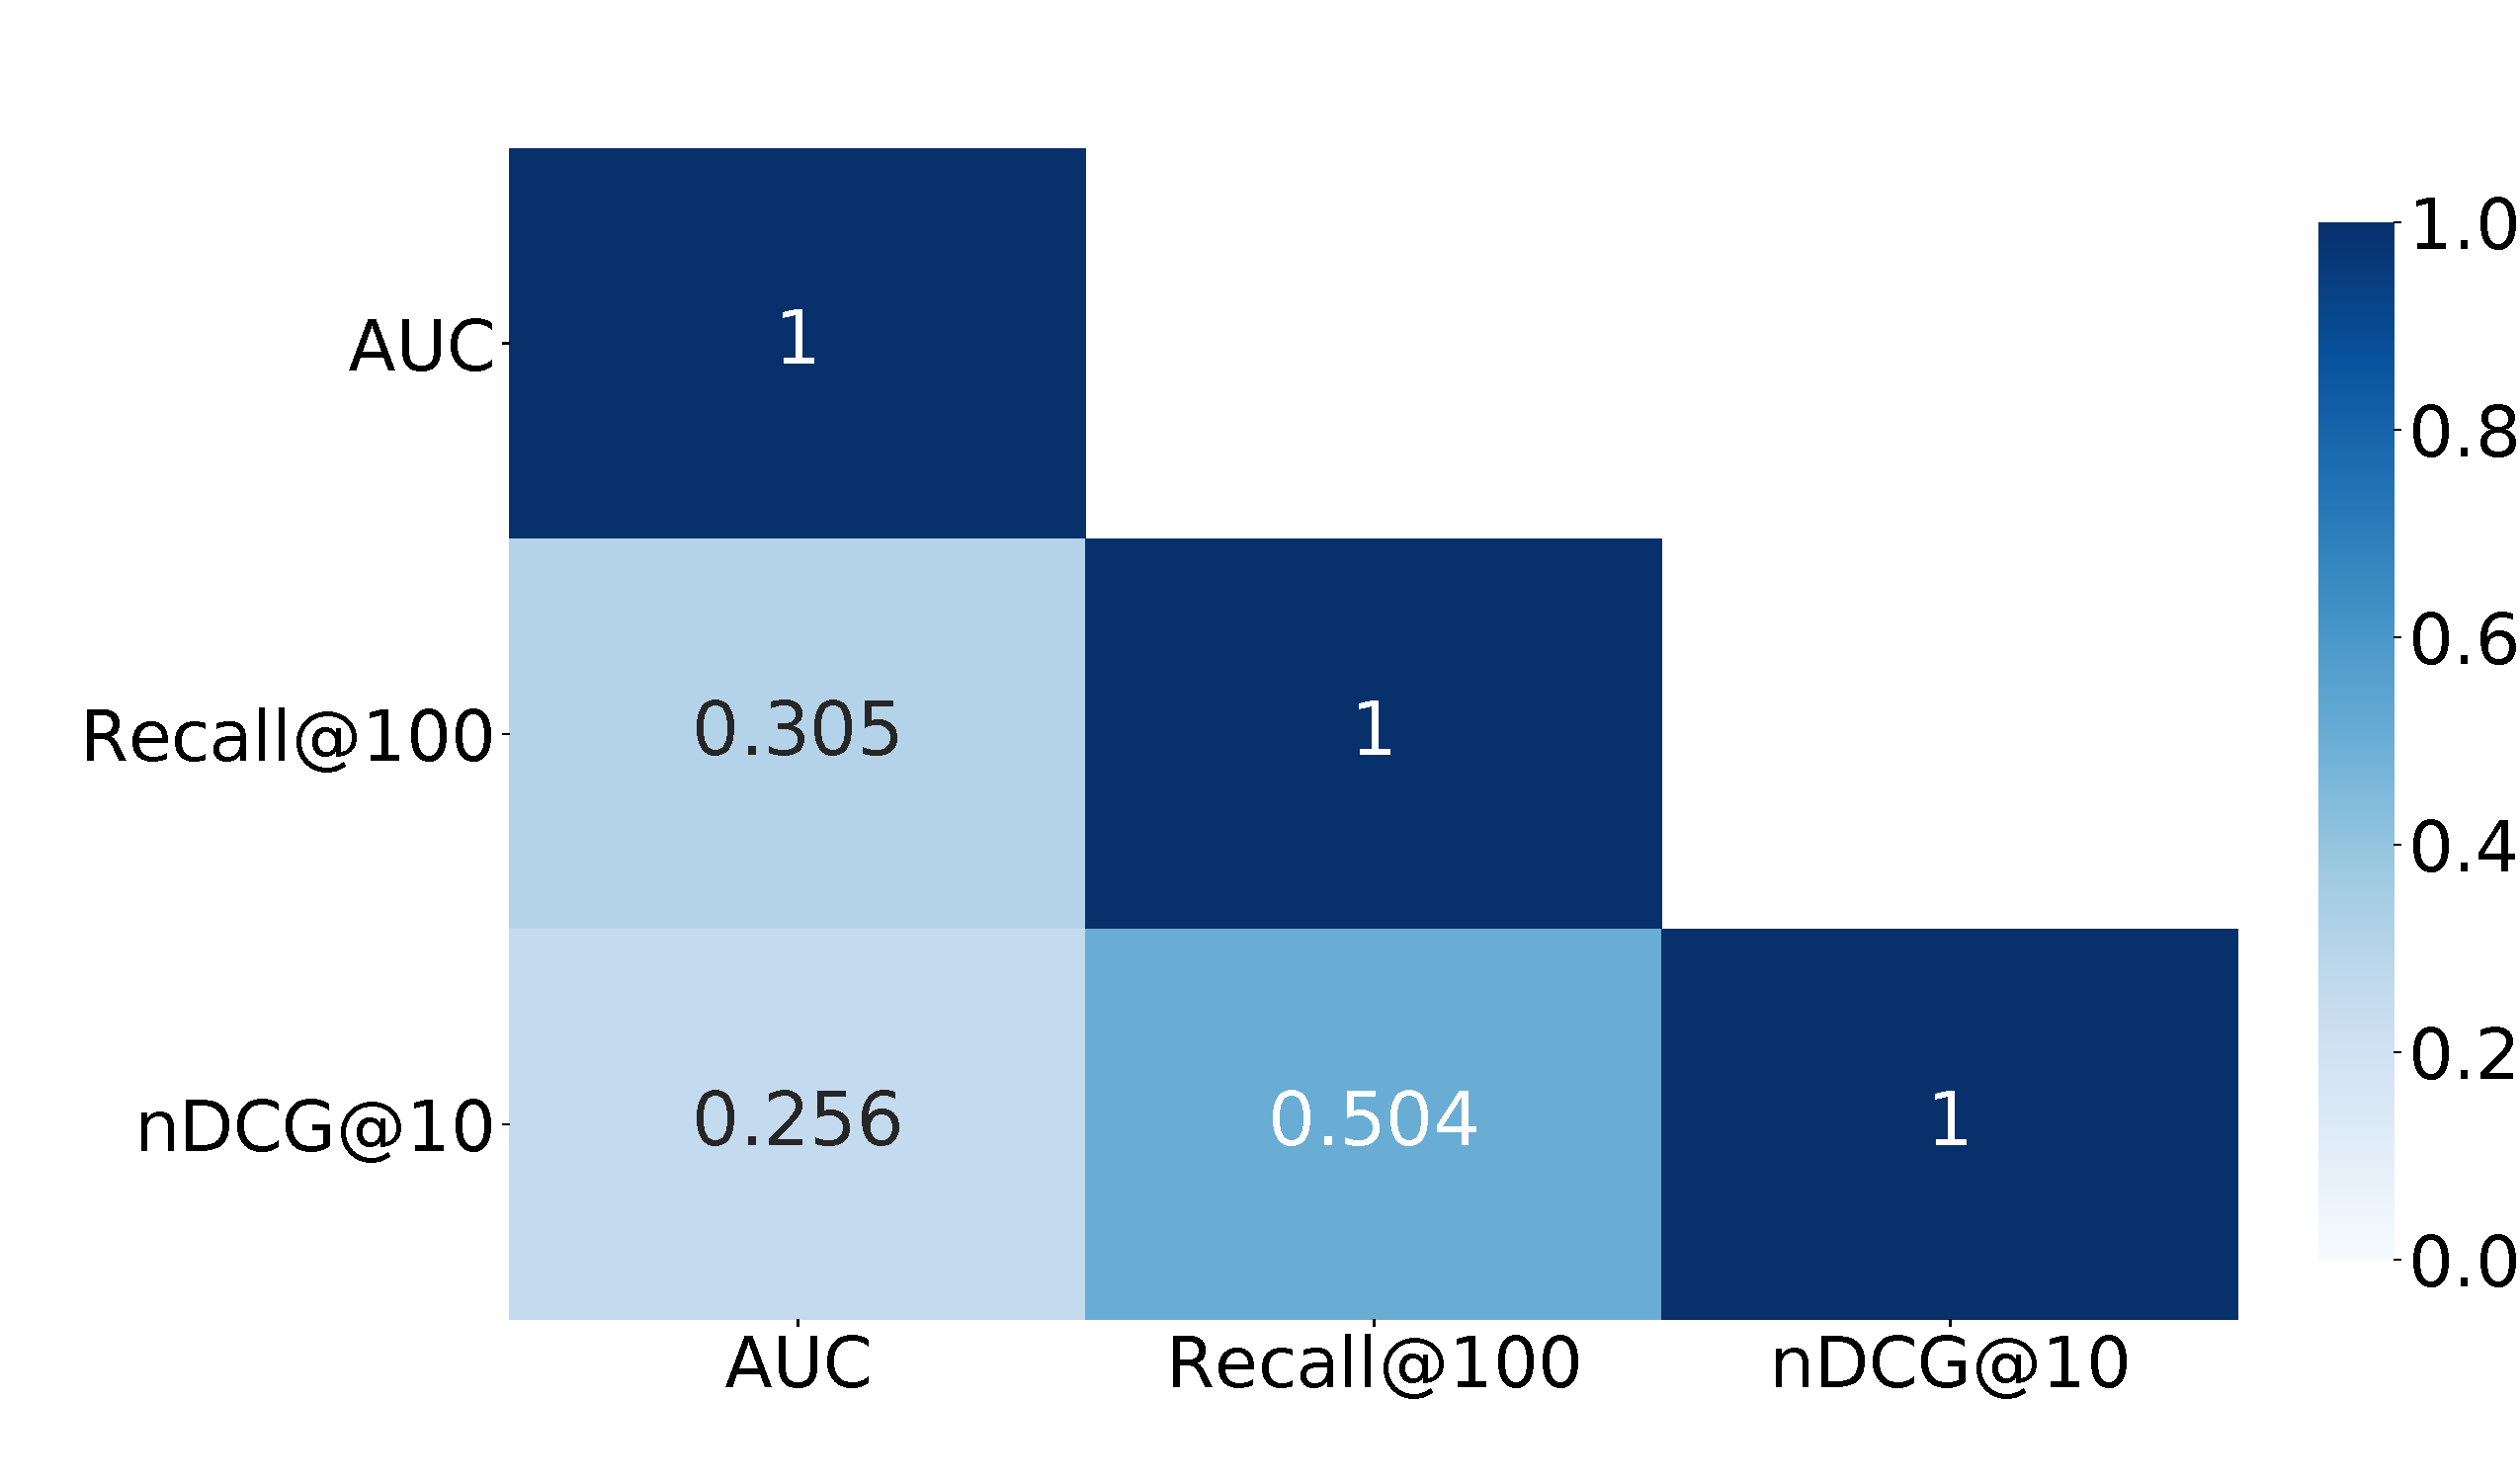
\includegraphics[width=\linewidth]{figures/metric_correlation.pdf}
%     \vspace{-0.92cm}
%     \caption{Average Kendall's Tau amongst the rankings of algorithms over different metrics.}
%     \label{metric_correlation}
%     \vspace{-0.5cm}
% \end{wrapfigure}
% \subsubsection{How do different metrics correlate with each other? \ \ } \ns{Check if we need to change this figure.} In an attempt to better understand how well do the three different implicit and sequential feedback metrics (\cref{feedback_types}) agree with each other, we visualize the average correlation between the algorithm rankings for each metric pair in \cref{metric_correlation}. To be precise, we compute the correlation between metric$_1$ and metric$_2$ as the Kendall's Tau between the ranked list of algorithms on metric$_1$ and metric$_2$ averaged over all datasets, sampling strategies and \% data sampled. We first observe that all three metrics correlate positively with each other. Finally, the AUC metric correlates less significantly with both Recall and nDCG than the correlation amongst Recall and nDCG.